\documentclass[10pt,landscape,a4paper]{article}
%\usepackage[utf8]{inputenc}
%\usepackage[ngerman]{babel}
\usepackage[normalem]{ulem}
\usepackage{tikz}
\usetikzlibrary{shapes,positioning,arrows,fit,calc,graphs,graphs.standard}
\usepackage[nosf]{kpfonts}
\usepackage[t1]{sourcesanspro}
%\usepackage[lf]{MyriadPro}
%\usepackage[lf,minionint]{MinionPro}
\usepackage{multicol}
\usepackage{wrapfig}
\usepackage[top=0mm,bottom=1mm,left=0mm,right=1mm]{geometry}
\usepackage[framemethod=tikz]{mdframed}
\usepackage{microtype}
%\usepackage{physics}
\usepackage{tabularx}
\usepackage{hhline}
\usepackage{makecell}
\usepackage{mathtools}

\usepackage{listings}

\DeclarePairedDelimiter{\ceil}{\lceil}{\rceil}

\newcommand\codeblue[1]{\textcolor{blue}{\code{#1}}}

\usepackage{lastpage}
\usepackage{datetime}
\yyyymmdddate
\renewcommand{\dateseparator}{-}
\let\bar\overline

\definecolor{myblue}{cmyk}{1,.72,0,.38}

\def\firstcircle{(0,0) circle (1.5cm)}
\def\secondcircle{(0:2cm) circle (1.5cm)}

\colorlet{circle edge}{myblue}
\colorlet{circle area}{myblue!5}

\tikzset{filled/.style={fill=circle area, draw=circle edge, thick},
outline/.style={draw=circle edge, thick}}

\pgfdeclarelayer{background}
\pgfsetlayers{background,main}

%\everymath\expandafter{\the\everymath \color{myblue}}
%\everydisplay\expandafter{\the\everydisplay \color{myblue}}


\renewcommand{\baselinestretch}{.8}
\pagestyle{empty}

\global\mdfdefinestyle{header}{%
  linecolor=gray,linewidth=1pt,%
  leftmargin=0mm,rightmargin=0mm,skipbelow=0mm,skipabove=0mm,
}

\newcommand{\header}{
  \begin{mdframed}[style=header]
    \footnotesize
    \sffamily
    CS2106 Midterms Cheatsheet v1.1 (\today)\\
    by~Julius Putra Tanu Setiaji,~page~\thepage~of~\pageref{LastPage}
  \end{mdframed}
}

\let\counterwithout\relax
\let\counterwithin\relax
\usepackage{chngcntr}

\usepackage{verbatim}

\usepackage{etoolbox}
\makeatletter
\preto{\@verbatim}{\topsep=0pt \partopsep=0pt }
\makeatother

\counterwithin*{equation}{section}
\counterwithin*{equation}{subsection}
\usepackage{enumitem}
\newlist{legal}{enumerate}{10}
\setlist[legal]{label*=\arabic*.,leftmargin=2.5mm}
\setlist[itemize]{leftmargin=3mm}
\setlist[enumerate]{leftmargin=3.5mm}
\setlist{nosep}
\usepackage{minted}

\def\code#1{\texttt{#1}}

\newenvironment{descitemize} % a mixture of description and itemize
{\begin{description}[leftmargin=*,before=\let\makelabel\descitemlabel]}
{\end{description}}

\newcommand{\descitemlabel}[1]{%
  \textbullet\ \textbf{#1}%
}
\makeatletter



\renewcommand{\section}{\@startsection{section}{1}{0mm}%
  {.2ex}%
  {.2ex}%x
{\color{myblue}\sffamily\small\bfseries}}
\renewcommand{\subsection}{\@startsection{subsection}{1}{0mm}%
  {.2ex}%
  {.2ex}%x
{\sffamily\bfseries}}
\renewcommand{\subsubsection}{\@startsection{subsubsection}{1}{0mm}%
  {.2ex}%
  {.2ex}%x
{\rmfamily\bfseries}}



\def\multi@column@out{%
  \ifnum\outputpenalty <-\@M
    \speci@ls \else
  \ifvoid\colbreak@box\else
    \mult@info\@ne{Re-adding forced
    break(s) for splitting}%
    \setbox\@cclv\vbox{%
      \unvbox\colbreak@box
    \penalty-\@Mv\unvbox\@cclv}%
  \fi
  \splittopskip\topskip
  \splitmaxdepth\maxdepth
  \dimen@\@colroom
  \divide\skip\footins\col@number
  \ifvoid\footins \else
    \leave@mult@footins
  \fi
  \let\ifshr@kingsaved\ifshr@king
    \ifvbox \@kludgeins
      \advance \dimen@ -\ht\@kludgeins
      \ifdim \wd\@kludgeins>\z@
        \shr@nkingtrue
      \fi
    \fi
    \process@cols\mult@gfirstbox{%
      %%%%% START CHANGE
      \ifnum\count@=\numexpr\mult@rightbox+2\relax
        \setbox\count@\vsplit\@cclv to \dimexpr \dimen@-1cm\relax
        \setbox\count@\vbox to \dimen@{\vbox to 1cm{\header}\unvbox\count@\vss}%
      \else
        \setbox\count@\vsplit\@cclv to \dimen@
      \fi
      %%%%% END CHANGE
      \set@keptmarks
      \setbox\count@
      \vbox to\dimen@
      {\unvbox\count@
        \remove@discardable@items
    \ifshr@nking\vfill\fi}%
    }%
    \setbox\mult@rightbox
    \vsplit\@cclv to\dimen@
    \set@keptmarks
    \setbox\mult@rightbox\vbox to\dimen@
    {\unvbox\mult@rightbox
      \remove@discardable@items
  \ifshr@nking\vfill\fi}%
    \let\ifshr@king\ifshr@kingsaved
  \ifvoid\@cclv \else
    \unvbox\@cclv
    \ifnum\outputpenalty=\@M
  \else
    \penalty\outputpenalty
  \fi
  \ifvoid\footins\else
    \PackageWarning{multicol}%
    {I moved some lines to
      the next page.\MessageBreak
      Footnotes on page
    \thepage\space might be wrong}%
  \fi
  \ifnum \c@tracingmulticols>\thr@@
\hrule\allowbreak \fi
  \fi
  \ifx\@empty\kept@firstmark
    \let\firstmark\kept@topmark
    \let\botmark\kept@topmark
  \else
    \let\firstmark\kept@firstmark
    \let\botmark\kept@botmark
  \fi
  \let\topmark\kept@topmark
  \mult@info\tw@
  {Use kept top mark:\MessageBreak
    \meaning\kept@topmark
    \MessageBreak
    Use kept first mark:\MessageBreak
    \meaning\kept@firstmark
    \MessageBreak
    Use kept bot mark:\MessageBreak
    \meaning\kept@botmark
    \MessageBreak
    Produce first mark:\MessageBreak
    \meaning\firstmark
    \MessageBreak
    Produce bot mark:\MessageBreak
    \meaning\botmark
  \@gobbletwo}%
  \setbox\@cclv\vbox{\unvbox\partial@page
  \page@sofar}%
  \@makecol\@outputpage
  \global\let\kept@topmark\botmark
  \global\let\kept@firstmark\@empty
  \global\let\kept@botmark\@empty
  \mult@info\tw@
  {(Re)Init top mark:\MessageBreak
    \meaning\kept@topmark
  \@gobbletwo}%
  \global\@colroom\@colht
  \global \@mparbottom \z@
  \process@deferreds
\@whilesw\if@fcolmade\fi{\@outputpage
    \global\@colroom\@colht
  \process@deferreds}%
  \mult@info\@ne
  {Colroom:\MessageBreak
    \the\@colht\space
    after float space removed
  = \the\@colroom \@gobble}%
  \set@mult@vsize \global
  \fi}
  \global\let\tikz@ensure@dollar@catcode=\relax

  \def\mathcolor#1#{\@mathcolor{#1}}
  \def\@mathcolor#1#2#3{%
    \protect\leavevmode
    \begingroup
    \color#1{#2}#3%
    \endgroup
  }

  \makeatother
  \setlength{\parindent}{0pt}

  \setminted{tabsize=2, breaklines}
  % Remove belowskip of minted
  \setlength\partopsep{-\topsep}


  \newcolumntype{a}{>{\hsize=1.5\hsize}X}
  \newcolumntype{b}{>{\hsize=.25\hsize}X}

  \setlength\columnsep{1.5pt}
  \setlength\columnseprule{0.1pt}
\begin{document}
\setlength{\abovedisplayskip}{0pt}
\setlength{\belowdisplayskip}{0pt}

\scriptsize
\begin{multicols*}{4}
  \raggedcolumns
  \section{Introduction to OS}
  \textbf{Motivation} for OS: Manage resources and coordination (process sync, resource sharing), Simplify programming (abstraction of hardware, convenient services), Enforce usage policies, Security and protection, User program portability: across different hardware, Efficiency: Sophisticated implementations optimised for particular usage and hardware.
  \subsection{OS Structures}
  \subsubsection{Monolithic}
  \begin{itemize}
    \item Kernel is one BIG special program, various services and components are integral part
    \item Good SE principles with modularisation, separation of interfaces and implementation
    \item \textbf{Advantages}: Well understood, Good performance
    \item \textbf{Disadvantages}: Highly coupled components, Usually devolved into very complicated internal structure
  \end{itemize}
  \subsubsection{Microkernel}
  \begin{itemize}
    \item Kernel is very small \& clean, only provides basic and essential facilities: IPC, address space \& thread management, etc.
    \item \textbf{Higher level services} built on top of the basic facilities, run as server process outside of the OS, using IPC to communicate
    \item \textbf{Advantages}: Kernel is generally more robust \& extensible, better isolation \& protection between kernel \& high level services.
    \item \textbf{Disadvantages}: Lower performance
  \end{itemize}
  \subsection{Virtual Machine \textmd{also known as }Hypervisor}
  A software emulation of hardware -- \textbf{virtualisation} of underlying hardware (illusion of complete hardware).
  \begin{itemize}
    \item \textbf{Type 1 Hypervisor}:\\
      Provides individual VMs to guest OS's (e.g. IBM VM/370)
    \item \textbf{Type 2 Hypervisor}:\\
      Runs in host OS, guest OS runs inside VM (e.g. VMware)
  \end{itemize}

  \section{Process Abstraction}
  \subsection{Process Abstraction}
  \begin{itemize}
    \item \textbf{Process} = a dynamic abstraction for executing program
    \item Information required to describe a running program (Memory context, hardware context, OS context)
    \item An executable binary consists of two major components: instructions and data
    \item During execution, more information:
    \begin{itemize}
      \item \textbf{Memory context}: text, data, stack, heap
      \item \textbf{Hardware context}: General Purpose Registers, Program Counter, Stack Pointer, Stack FP, ...
      \item \textbf{OS context}: PID, Process state, ...
    \end{itemize}
  \end{itemize}
  \begin{tabular}{l}
    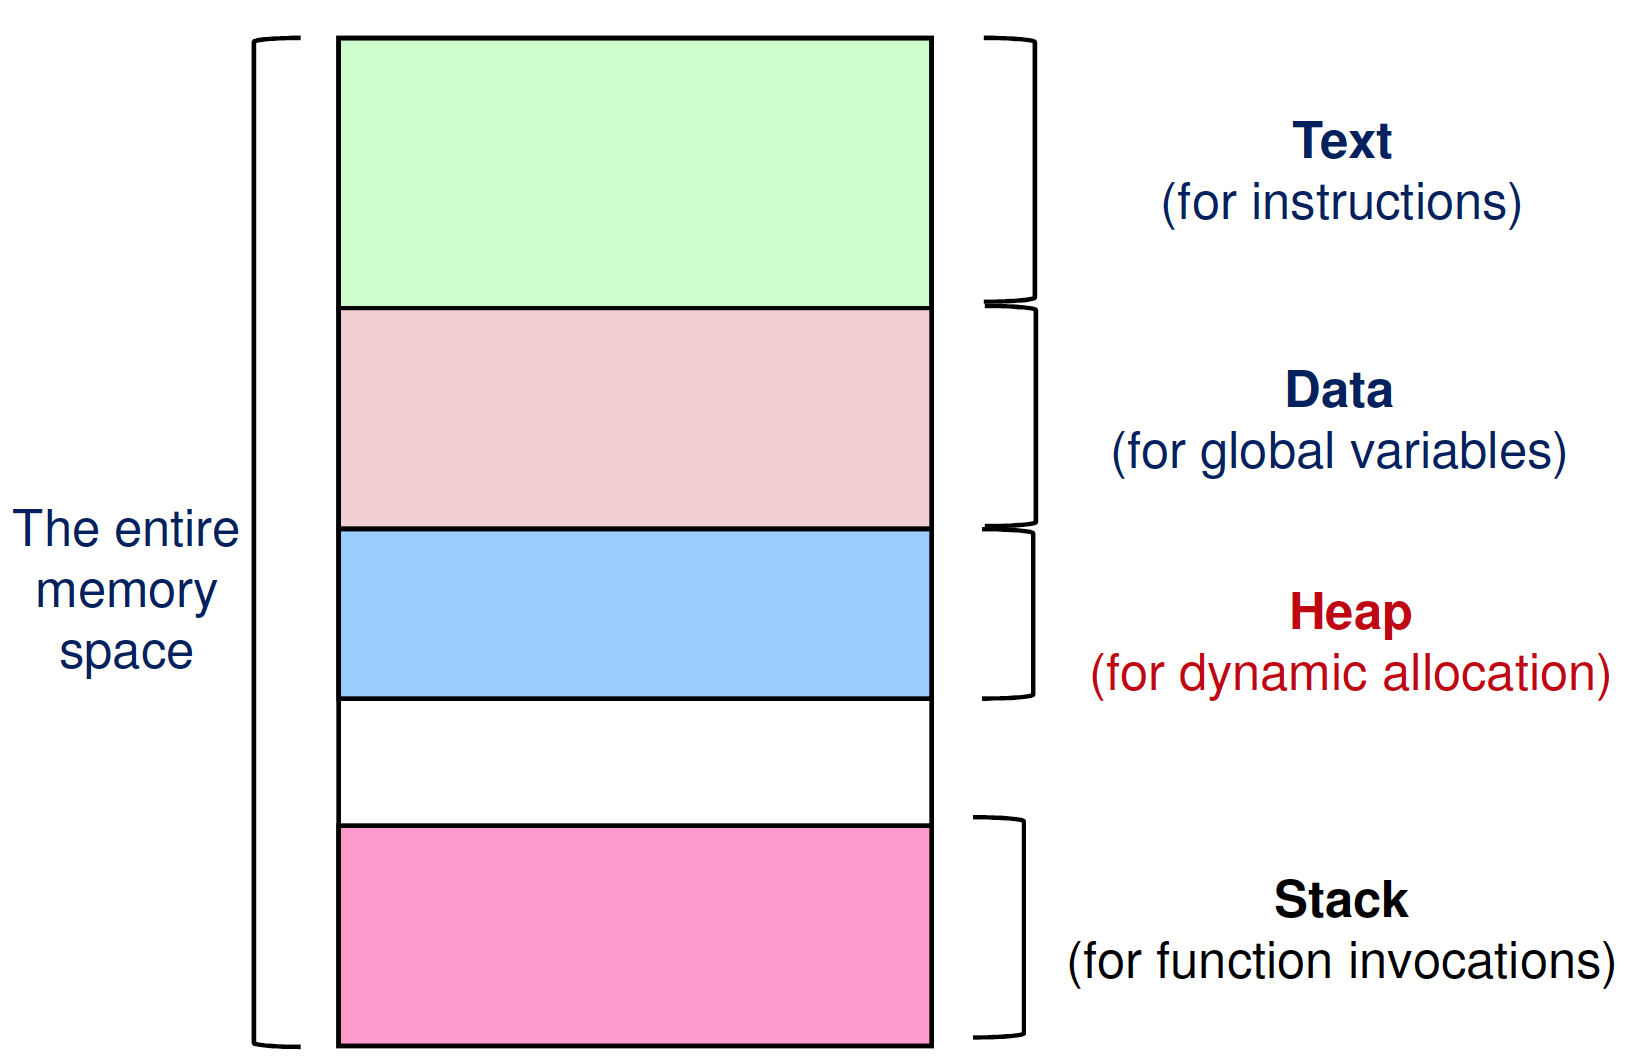
\includegraphics[width=0.5\linewidth]{stack-memory}
  \end{tabular}
  \begin{tabularx}{0.45\columnwidth}{X}
    Note: stack grow upwards in this case
  \end{tabularx}
  
  \subsection{Stack Memory}
  \begin{itemize}
    \item New memory region to store information of a function invocation
    \item Described by a \textbf{stack frame}, containing: Return address of the caller (PC, old SP), Arguments for the function, Storage for local variables, Frame Pointer, Saved Registers
    \item \textbf{Stack Pointer} = The top of stack region (first unused location)
    \item \textbf{Frame Pointer} = points to a fixed location in a stack frame
    \item \textbf{Saved Registers} = memory to temporarily hold GPR value during \textbf{register spilling}
  \end{itemize}
  \subsubsection{Function Call Convention}
  E.g. On executing function call, \textbf{Caller}: Pass parameters with registers and/or stack, Save Return PC on stack; \textbf{Callee}: Save the old FP, SP, Allocate space for local vars on stack, adjust SP (Stack Pointer) \\
  On returning from function call, \textbf{Callee}: Restore saved registers, FP, SP; \textbf{Caller}: Continues execution
  \subsection{Dynamically Allocated Memory}
  Using a separate \textbf{heap memory region}
  \subsection{Process Identification \& Process State}
  \begin{itemize}
    \item Using process ID \textbf{(PID)}, a unique number among the processes.
    \item OS dependent: Are PID's reused? Are there reserved PID's? Does it limit max number of processes?
  \end{itemize}
  \begin{tabular}{l}
    \textbf{5 State Process Model}:\\
    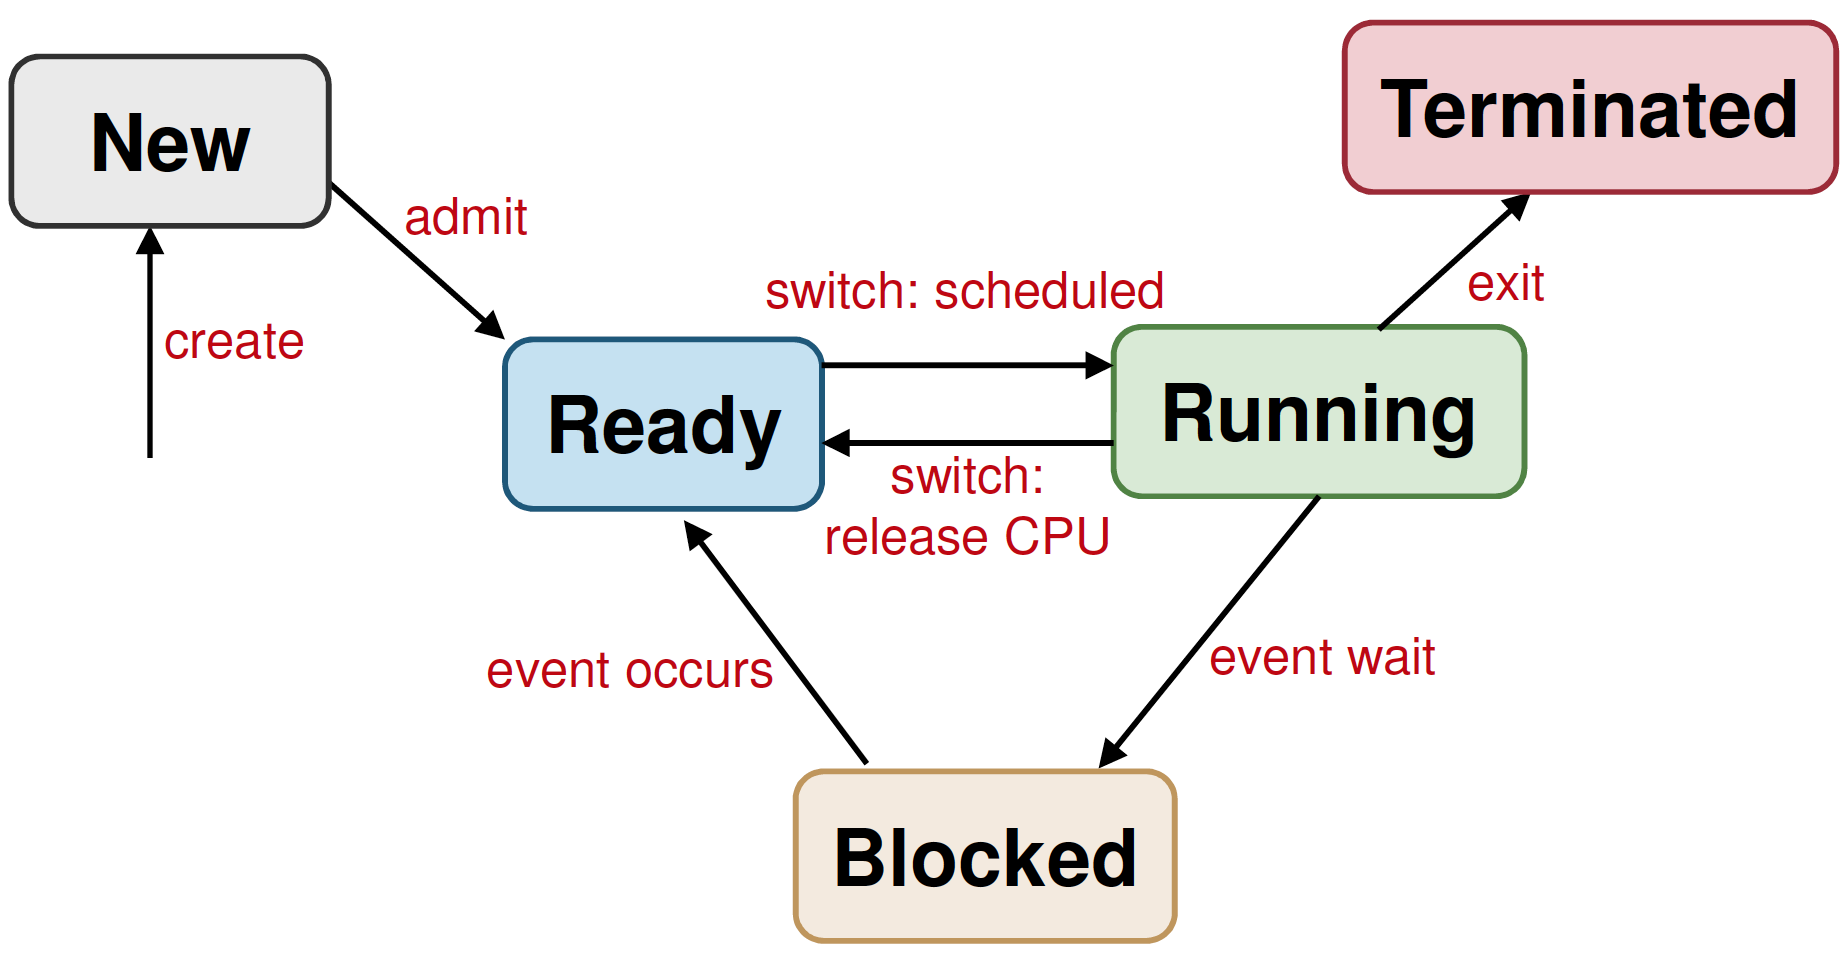
\includegraphics[width=0.55\linewidth]{process-state}
  \end{tabular}
  \begin{tabularx}{0.4\columnwidth}{X}
  \begin{itemize}
    \item \textbf{Process State} = indication of the execution status
  \end{itemize}
  \end{tabularx}
  \begin{enumerate}
    \item \textbf{New}: process created, may still be initialising, not yet ready
    \item \textbf{Ready}: process is waiting to run
    \item \textbf{Running}: process being executed on CPU
    \item \textbf{Blocked}: process waiting, can't execute till event is available
    \item \textbf{Terminated}: process finished execution, may require OS cleanup
  \end{enumerate}
  \textbf{Transitions}:
  \begin{itemize}
    \item nil -> New (Create)
    \item New -> Ready (Admit): Process ready to be scheduled
    \item Ready -> Running (Switch): Process selected to run
    \item Running -> Ready (Switch): Process gives up CPU voluntarily or preempted by scheduler
    \item Running -> Blocked (Event wait): e.g. syscall, waiting for I/O, ...
    \item Blocked -> Ready (Event occurs)
  \end{itemize}
  \subsection{Process Table \& Process Control Block}
  \begin{tabularx}{0.42\columnwidth}{X}
    \begin{itemize}
      \item \textbf{PCB/Process Table Entry} = entire execution context for a process
      \item \textbf{Process Table} =  maintains PCB for all processes, stored as one table
      \item Issues: Scalability, Efficiency
    \end{itemize}
  \end{tabularx}
  \begin{tabular}{l}
    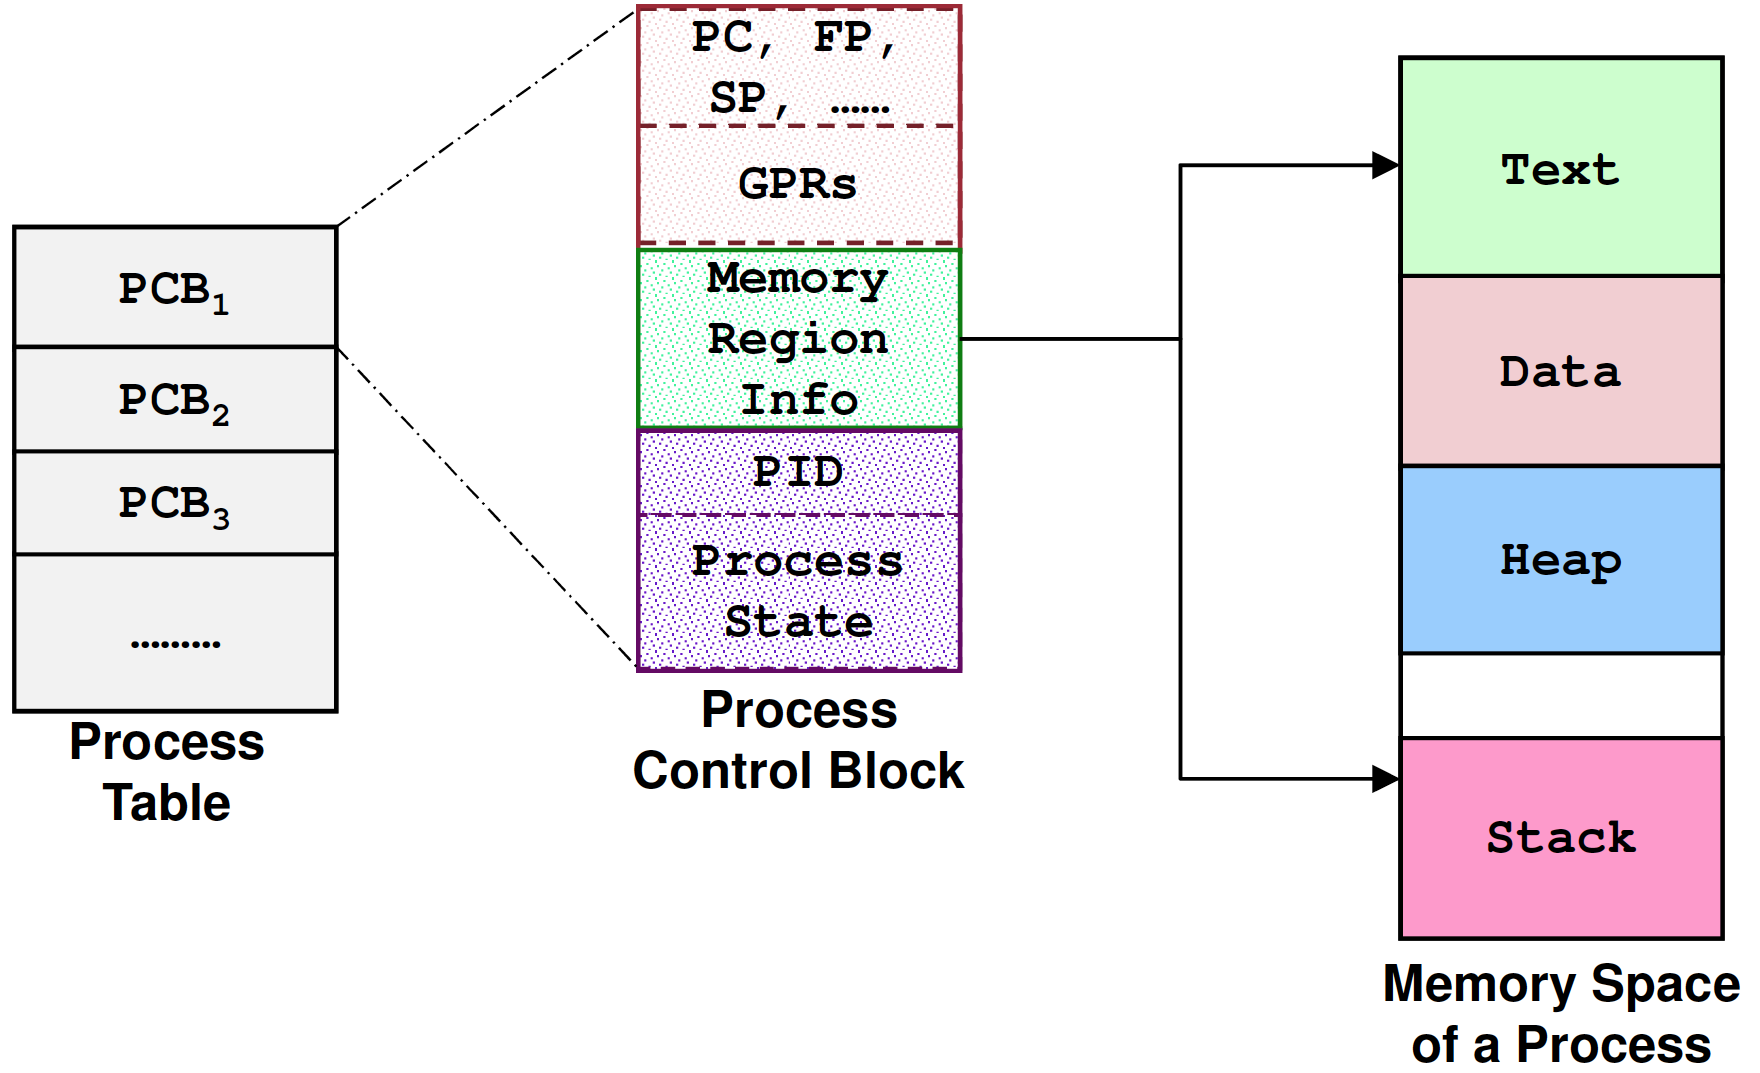
\includegraphics[width=0.55\linewidth]{process-table}
  \end{tabular}
  \subsection{System Calls}
  \begin{itemize}
    \item API to OS -- different from normal function call in that have to change from user mode -> kernel mode
    \item General System Call Mechanism:
    \begin{enumerate}
      \item User program invokes the library call (using normal function call mechanism)
      \item Library call places the system call number in a designated location (e.g. register)
      \item Library call executes a special instruction to switch user -> kernel mode (commonly known as TRAP)
      \item In kernel mode, the dispatching to the appropriate system call handler by dispatcher
      \item System call handler is executed
      \item System call handler ended, control return to library call, switch kernel -> user mode
      \item Library call return to user program via normal function return mechanism
    \end{enumerate}
  \end{itemize}
  \subsection{Exception \& Interrupt}
  \textbf{Exception}:
  \begin{itemize}
    \item Synchronous, occurring due to program execution
    \item Effect: have to execute an \textbf{exception handler}, similar to a forced function call
  \end{itemize}
  \textbf{Interrupt}:
  \begin{itemize}
    \item External events interrupting execution, usually hardware-related
    \item Asynchronous, occurring independent of program execution
    \item Effect: execution is suspended, have to execute \textbf{interrupt handler}
  \end{itemize}
  \subsection{Process Abstraction: Unix}
  \begin{itemize}
    \item \mintinline{C}{int fork();} duplicate current executable, returns PID of newly created process (for parent) or 0 (for child)
    \item \mintinline{C}{int execl(const char *path, const char *arg0, ..., const char *argN, NULL);} replaces current executing process image, does not return unless error. Will not exit on error.
    \item \mintinline{C}{void exit(int status);} \texttt{status} is 0 for normal, else problematic. Does not return.
    \item \mintinline{C}{int wait(int *status);} returns the PID of terminated child, status stores exit status. Blocking.
  \end{itemize}
  \textbf{Zombie process} = (1) parent terminates before child -- \texttt{init} becomes pseudo-parent, who will call \texttt{wait} on children (2) child process terminates but parent did not call \texttt{wait} -- child becomes zombie, can fill up processs table
  \section{Process Scheduling}
  3 categories of \textbf{processing environment}: (1) \textbf{Batch Processing}: no user, no interaction, no need to be responsive, (2) \textbf{Interactive}: with active user interacting, need to be responsive, consistent in response time, (3) \textbf{Real-time Processing}: deadline to meet, usually periodic process
  \subsection{Criteria for Scheduling Algorithms}
  \begin{itemize}
    \item \textbf{Fairness}: fair share of CPU time, no starvation
    \item \textbf{Balance}: all parts of the computing system should be utilised
  \end{itemize}
  \subsection{Types of scheduling policies}
  \begin{itemize}
    \item \textbf{Non-preemptive (cooperative)} -- a process stays scheduled until it blocks/gives up the CPU voluntarily
    \item \textbf{Preemptive}: A process is given a fixed time quota to run (possible to block or yield early), at the end of the time quota, the running process is suspended.
  \end{itemize}
  \subsection{Scheduling a process}
  \begin{enumerate}
    \item Scheduler is triggered (OS takes over)
    \item If context switch is needed: context of current running process is saved, placed on blocked/ready queue
    \item Pick a suitable process \textbf{P} to run based on scheduling algorithm
    \item Setup the context for \textbf{P}
    \item Let process \textbf{P} run
  \end{enumerate}
  \subsection{Scheduling for Batch Processing}
  Criteria:
  \begin{itemize}
    \item \textbf{Turnaround time}: Total time taken
    \item \textbf{Throughput}: Rate of task completion
    \item \textbf{CPU Utilisation}: \% of time when CPU is working on a task
  \end{itemize}
  \subsubsection{First-Come First-Served (FCFS)}
  \begin{itemize}
    \item Tasks are stored on a FIFO queue based on arrival time. Pick the head of queue to run until (task is done OR task is blocked). Blocked task removed from queue, when it is ready again, placed at back of queue like a newly arrived task.
    \item \textbf{Guaranteed} to have no starvation: no of tasks in front of task X in FIFO is always decreasing -> task X will get its chance eventually.
    \item Shortcoming: \textbf{Convoy Effect} -- due to non-preemptiveness, one slow process (CPU intensive) slows down the performance of the entire set of processes.
  \end{itemize}
  \subsubsection{Shortest Job First (SJF)}
  \begin{itemize}
    \item Select the task with the smallest total CPU time, thus \textbf{guaranteeing} smallest average waiting time.
    \item Shortcomings: Need to know total CPU time for a task in advance (have to guess if not available), starvation is possible (biased towards short jobs, long jobs may never get a chance)
    \item Predicting CPU Time, common approach (\textbf{Exponential Average}):\\
    $\text{Predicted}_{n+1} = \alpha \text{Actual}_n + (1-\alpha)\text{Predicted}_n$, where $\alpha =$ degree of weighting decrease, higher $\alpha$ discounts older observations faster
  \end{itemize}
  \subsubsection{Shortest Remaining Time (SRT)}
  \begin{itemize}
    \item Select job with shortest remaining (or expected) time.
    \item Variation of SJF that is preemptive and uses remaining time.
    \item New job with shorter remaining time can preempt currently running job
    \item Provide good service for short jobs even when they arrive late
  \end{itemize}

  \subsection{Scheduling for Interactive Systems}
  \begin{itemize}
    \item 
    Criteria:
    \begin{itemize}
      \item \textbf{Response time}: Time between request and response by system
      \item \textbf{Predictability}: Lesser variation in response time
    \end{itemize}
    \item Preemptive scheduling algorithms are used to ensure good response time, thus scheduler needs to run periodically.
    \item \textbf{Timer interrupt} = interrupt that goes off periodically based on hardware clock
    \item Timer interrupt handler \textbf{invokes OS scheduler}.
    \item \textbf{Interval of Timer Interrupt (ITI)} typically 1-10ms
    \item \textbf{Time Quantum} = execution duration given to a process, can be constant/variable, must be multiple of ITI (commonly 5-100ms)
  \end{itemize}
  \subsubsection{Round Robin (RR)}
  \begin{itemize}
    \item Tasks stored in a FIFO queue, pick task from head of queue until (time quantum elapsed OR task gives up CPU voluntarily OR task blocks)
    \item Basically a preemptive version of FCFS
    \item Response time guarantee: given $n$ tasks and quantum $q$, time before a task get CPU is bounded by $(n-1)q$
    \item Choice of time quantum: big = better CPU util, longer waiting time; small = bigger overhead (worse CPU util) but shorter waiting time
  \end{itemize}
  \subsubsection{Priority Scheduling}
  \begin{itemize}
    \item Assign a priority value to all tasks, select task with highest priority value.
    \item Preemptive: highest priority process can preempt running process with lower priority
    \item Non-preemptive: late coming high priority process has to wait for next round of scheduling
    \item \textbf{Shortcomings}: Low priority process can starve, worse in preemptive variant
    \item \textbf{Possible solutions}: Decrease the prioty of currently running process after every time quantum, Given the current running process a time quantum -- this process not considered in the next round of scheduling
    \item Generally hard to guarantee/control exact amount of CPU time given to a process
    \item \textbf{Priority Inversion}: 3 processes, priorities Hi, Mi, Lo. L locks resource, M pre-empts L, A arrives and tries to lock same resource as L. Then M continues executing although H has higher priority.
  \end{itemize}
  \subsubsection{Multi-level Feedback Queue (MLFQ)}
  \begin{itemize}
    \item Adaptive, minimising both response time for IO-bound and turnaround time for CPU-bound
    \item Rules:
    \begin{itemize}
      \item Priority(A) $>$ Priority(B) -> A runs
      \item Priority(A) == Priority(B) -> A and B in RR
      \item New job -> highest priority
      \item If a job fully utilised its time slice -> priority reduced
      \item If a job gives up/blocks before it finishes the time slice -> priority retained
    \end{itemize}
    \item \textbf{Shortcomings}: (1) Starvation -- if there are too many interactive jobs, long-running jobs will starve, (2) gaming the scheduler by running for 99\% of time quantum, then relinquish the CPU, (3) a program may change its behaviour CPU-bound -> interactive
    \item Possible solution:
    \begin{itemize}
      \item \textbf{Priority boost}: after some time period S, move all jobs to the highest priority. Guaranteeing no starvation as highest priority -> RR, and the case when CPU-bound job has become interactive
      \item \textbf{Better accounting}: Once a job uses up its time allotment at a given level, its priority is reduced
    \end{itemize}
  \end{itemize}
  \subsubsection{Lottery Scheduling}
  \begin{itemize}
    \item Give out "lottery tickets" to processes. When a scheduling decision is needed, a ticket is chosen randomly among eligible tickets.
    \item In the long run, a process holding X\% of tickets can win X\% of the lottery held and use the resource X\% of the time.
    \item Reponsive: newly created process can participate in next lottery
    \item Good level of control: A process can be given lottery tickets to be distributed to its child process, an important process can be given more lottery tickets, each resource can have its own set of tickets (different proportion of usage per resource per task)
    \item Simple implementation
  \end{itemize}

  \section{Process Alternative -- Threads}
  \begin{itemize}
    \item Motivation:
    \begin{itemize}
      \item Process is expensive: under \texttt{fork()} model -- duplicate memory space and process context, context switch requires saving/restoration of process information
      \item Hard for independent processes to communicate with each other: independent memory space -- no easy way to pass information, requires Inter-Process Communication (IPC)
    \end{itemize}
    \item A traditional process has a single thread of control -- only one instruction of the whole program is executing at any one time. Instead, we add more threads of control such that multiple parts of the program are executing simultaneously conceptually.
  \end{itemize}
  \subsection{Process and Thread}
  \begin{itemize}
    \item A single process can have multiple threads
    \item Threads in the same process shares: \textbf{Memory Context} (text, data, heap), and \textbf{OS Context} (PID, other resources like files, etc.)
    \item Unique information needed for each thread: Identification (usually thread id), Registers (general purpose \& special), "stack"
    \item Process context switch involves: OS Context, Hardware Context, Memory Context
    \item Thread switch within the same process involves: Hardware context (registers, "stack" -- actually just changing FP and SP)
  \end{itemize}
  \subsection{Benefits}
  \begin{itemize}
    \item \textbf{Economy}: requires much less resources
    \item \textbf{Resource sharing}: no need for additional information passing mechanism
    \item \textbf{Responsiveness}: multithreaded programs can appear much more responsive
    \item \textbf{Scalability}: Multithreaded program can take advantage of multiple CPU's
  \end{itemize}
  \subsection{Problems}
  \begin{itemize}
    \item \textbf{System call concurrency} -- have to guarantee correctness and determine the correct behaviour
    \item \textbf{Process behaviour} -- impact on process operations, e.g. does \texttt{fork()} duplicate threads? If single thread executes \texttt{exit()}, hwo abut the whole process, etc.
  \end{itemize}
  \subsection{Thread Models}
  \begin{itemize}
    \item \textbf{User Thread}
    \begin{itemize}
      \item Implemented as a user library, a runtime system in the process handles thread operations
      \item Kernel is not aware of threads in the process.
      \item \textbf{Advantages}: Multithreaded program on ANY OS, thread operations are just library calls, more conigurable and flexible (such as customised thread scheduling policy)
      \item \textbf{Disadvantages}: OS is not aware of threads, scheduling is performed at process level. One thread blocked -> process blocked -> all threads blocked, cannot exploit multiple CPUs
    \end{itemize}
    \item \textbf{Kernel Thread}
    \begin{itemize}
      \item Implemented in the OS, thread operation as system calls.
      \item Thread-level scheduling is possible
      \item Kernel may make use of threads for its own execution
      \item \textbf{Advantages}: Kernel can schedule on thread level
      \item \textbf{Disadvantages}: Thread operation is a syscall (slower and more resource intensive), generally less flexible (used by all multithreaded programs -- many features: expensive, overkill for simple program, few features: not flexible enough for some)
    \end{itemize}
    \item \textbf{Hybrid Thread Model}:
    \begin{itemize}
      \item Have both kernel and user threads, OS schedule on kernel threads only, user thread can bind to a kernel thread.
      \item Great flexibility (can limit concurrency of any process/user)
    \end{itemize}
  \end{itemize}
  \subsection{Threads on Modern Processor (Intel Hyperthreading)}
  \begin{itemize}
    \item Threads started off as software mechanism: Userspace lib -> OS aware mechanism
    \item Hardware support on modern processors, supplying multiple sets of registers to allow threads to run natively and parallelly on the same core: \textbf{Simultaneous Multi-Threading (SMT)}
  \end{itemize}
  \subsection{POSIX Threads: \texttt{pthread}}
  \begin{itemize}
    \item Standard by IEEE, defining API and behaviour.
    \item \mintinline{C}{int pthread_create(pthread_t* tidCreated, const pthread_attr_t* threadAttributes, void* (*startRoutine) (void*), void* argForStartRoutine);}
    \item \mintinline{C}{int pthread_exit(void* exitValue)}
    \item \mintinline{C}{int pthread_join(pthread_t threadID, void **status);}
    \item except for \texttt{pthread\_exit}, return 0 = success
  \end{itemize}

  \section{Inter-Process Communication}
  \begin{itemize}
    \item 2 common IPC mechanisms: Shared-Memory \& Message Passing
    \item 2 Unix-specific IPC mechanisms: Pipe and Signal
  \end{itemize}
  \subsection{Shared-Memory}
  \begin{itemize}
    \item General idea: Process $p_1$ creates a shared memory region $M$, process $p_2$ attaches $m$ to its own memory space. $p_1$ and $p_2$ can now commmunicate suing memory region $M$
    \item OS involved only in creating and attaching shared memory region
    \item \textbf{Advantages}: Efficient (only initial steps involves OS), Ease of use (information of any type or size can be written easily)
    \item \textbf{Disadvantages}: Synchronisation (shared resource -> need to synchronise access), Implementation is usually harder
    \item In Unix: (1) create/locate shared memory region $M$, (2) Attach $M$ to process memory space, (3) Read/Write $M$, (4) Detach $M$ from memory space after use, (5) Destroy $M$ (only 1 process, can only destroy if $M$ is not attached)
  \end{itemize}
  \subsection{Message Passing}
  \begin{itemize}
    \item General idea: process $p_1$ prepares a message $M$ and send it to process $p_2$, $p_2$ receives the message $M$
    \item Message has to be stored in kernel memory space, every send/receive operation is a syscall
    \item \textbf{Advantages}: Portable (can be easily implemented on different processing environment), Easier synchronisation (using synchronous primitive)
    \item \textbf{Disadvantages}: Inefficient (usually requiring OS intervention), Harder to use (message usually limited in size and/or format)
  \end{itemize}
  \subsubsection{Naming \textmd{(how to identify the other party in the comm):}}
  \begin{itemize}
    \item \textbf{Direct Communication}
    \begin{itemize}
      \item Sender/receiver explicitly name the other party
      \item Characteristics: 1 link/pair of communicating processes, need to know the identity of the other party
    \end{itemize}
    \item \textbf{Indirect Communication}
    \begin{itemize}
      \item Message are sent to/received from message storage (known as mailbox or port)
      \item Characteristic: 1 mailbox can be shared among a number of processes
    \end{itemize}
  \end{itemize}
  \subsubsection{Synchronisation \textmd{(behaviour of the sending/receiving ops)}}
  \begin{itemize}
    \item \textbf{Blocking primitives} (synchronous): sender/receiver is blocked until message is received/has arrived
    \item \textbf{Non-blocking Primitive} (asynchronous): sender resume operation immediately, receiver either receive message if available or some indication that message is not ready yet.
  \end{itemize}
  \subsection{Unix Pipes}
  \begin{itemize}
    \item A communication channel with 2 ends, for reading and writing.
    \item A pipe can be shared between 2 processes (producer-consumer)
    \item Behaviour: like an anonymous file, FIFO (in-order access)
    \item Pipe functions as \textbf{circular bounded byte buffer with implicit synchronisation}: writers wait when buffer full, readers wait when buffer empty
    \item Variants: Multiple readers/writers, half-duplex (unidirectional) or full-duplex (bidirectional)
    \item \mintinline{C}{int pipe(int fd[]);} returns 0 = success. \mintinline{C}{fd[0]} reading end, \mintinline{C}{fd[1]} writing end
  \end{itemize}
  \subsection{Unix Signal}
  \begin{itemize}
    \item An async notification regarding an event sent to a process/thread
    \item Recipient of signal handle by a default set of handlers OR user-supplied handler
    \item Common signals in Unix: SIGKILL, SIGSTOP, SIGCONT, etc.
  \end{itemize}

  \section{Synchronization}
  \subsection{Race Condition}
  \begin{itemize}
    \item When 2/more processes execute concurrently in interleaving fashion AND share a modifiable resource resulting in non-deterministic execution.
    \item Solution: designate code segment with race condition as \textbf{critical section} where at any point in time only 1 process can execute.
  \end{itemize}
  \subsection{Critical Section}
  Properties of correct implementation:
  \begin{itemize}
    \item \textbf{Mutual Exclusion}: if a process is executing in critical section, all other processes are prevented from entering it
    \item \textbf{Progress}: If no process is in critical section, one of the waiting processes should be granted access
    \item \textbf{Bounded Wait}: After a process $p_i$ requests to enter the critical section, $\exists$ an upper-bound of number of times other processes can enter the critical section before $p_i$
    \item \textbf{Independence}: process not executing in critical section should never block other processes
  \end{itemize}
  Symptoms of incorrect synchronisation:
  \begin{itemize}
    \item \textbf{Deadlock}: all processes blocked -> no progress
    \item \textbf{Livelock}: processes keep changing state to avoid deadlock and make no other progress, typically processes are not blocked
    \item \textbf{Starvation}: some processes are blocked forever
  \end{itemize}
  \subsection{Implementations of Critical Section}
  \subsubsection{Test-and-set: an atomic instruction}
  \begin{itemize}
    \item Load the current content at \texttt{MemoryLocation} into \texttt{Register}, Stores a \texttt{1} into \texttt{MemoryLocation}
    \item Disadvantage: busy waiting -- wasteful use of processing power
  \end{itemize}
  \subsubsection{Peterson's Algorithms}
  \begin{minted}{C}
bool flag[2] = {false, false};
int turn;
  \end{minted}
  \begin{multicols*}{2}
    \begin{minted}{C}
flag[0] = true;
turn = 1;
while (flag[1] && turn == 1) {
  // busy wait
}
// critical section
flag[0] = false;
    \end{minted}
    \begin{minted}{C}
flag[1] = true;
turn = 0;
while (flag[1] && turn == 0) {
  // busy wait
}
// critical section
flag[1] = false;
    \end{minted}
  \end{multicols*}
  Disadvantages:
  \begin{itemize}
    \item \textbf{Busy Waiting}, wasteful use of processing power
    \item \textbf{Low level}: higher-level programming construct desirable to simplify mutex and less error prone
    \item \textbf{Not general}: general synchronisation mechanism is desirable, not just mutex
  \end{itemize}
  \subsubsection{Semaphore}
  A generalised synchronisation mechanism, providing a way to block a number of processes and a way to unblock one/more sleeping process(es)
  \begin{itemize}
    \item \texttt{wait(S)}: if $S$ is (+)-ve, decrement. If $S$ is now (-)ve, go to sleep
    \item \texttt{signal(S)}: increment S, if pre-increment $S$ negative, wakes up 1 sleeping process
  \end{itemize}
  \textbf{Properties}
  \begin{itemize}
    \item Given $S_\text{initial} \geq 0$, where \#signal(S) = no of \texttt{signal()} executed, \#wait(S) = no of \texttt{wait()} completed
    \item \textbf{Invariant}: $S_\text{current} = S_\text{initial} +$ \#signal(S) $- $ \#wait(S)
  \end{itemize}
  Binary semaphore, $S = 0$ or $1$ known as mutex (mutual exclusion)\\
  Deadlock still possible 
  \subsection{Classical Synchronisation Problems}
  \begin{itemize}
    \item \textbf{Producer-Consumer}: produce only if buffer not full, consume only if buffer not empty
    \item \textbf{Reader-Writers}: writer exclusive access, reader can share
    \item \textbf{Dining Philosophers}: assign partial order to the resources, establishing convention that all resources will be requested in order. E.g. label forks 1-5, and always pick up lower-numbered fork first.
  \end{itemize}
  \subsection{Synchronisation Implementations}
  \begin{itemize}
    \item POSIX semaphores
    \item pthread\_mutex\_t: \texttt{pthread\_mutex\_lock}, \texttt{pthread\_mutex\_unlock}
    \item pthread\_cond\_t: \texttt{pthread\_cond\_wait}, \texttt{pthread\_cond\_signal}, \texttt{pthread\_cond\_broadcast}
  \end{itemize}
  
\end{multicols*}
\end{document}
